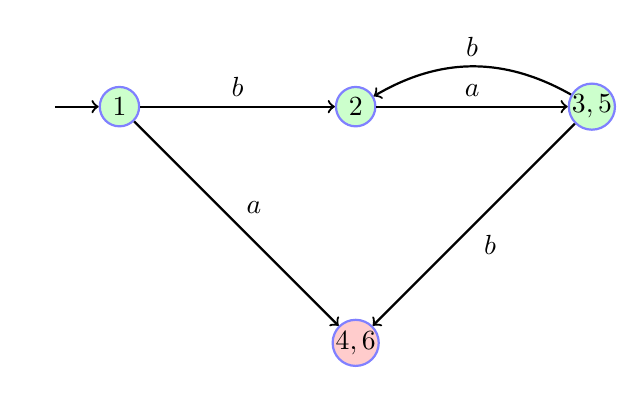
\begin{tikzpicture}



	\node 	(e0)		at	(-1,0) 	[circle, thick]{};

	\node 	(e1)		at	(0,0) 	[circle, thick, draw=blue!50,fill=green!20,inner sep=0pt,minimum size=.5cm]{$1$};

	\node 	(e2)		at	(3,0) 	[circle, thick, draw=blue!50,fill=green!20,inner sep=0pt,minimum size=.5cm]{$2$};


	\node 	(e3)		at	(6,0) 	[circle, thick, draw=blue!50,fill=green!20,inner sep=0pt,minimum size=.5cm]{$3,5$};



%	\node 	(e4)		at	(0,-4) 	[circle, thick, draw=blue!50,fill=green!20,inner sep=0pt,minimum size=.5cm]{$4$};


%	\node 	(e5)		at	(3,-4) 	[circle, thick, draw=blue!50,fill=green!20,inner sep=0pt,minimum size=.5cm]{$5$};

	\node 	(e6)		at	(3,-3) 	[circle, thick, draw=blue!50,fill=red!20,inner sep=0pt,minimum size=.5cm]{$4,6$};

	\draw[->, thick]	(e0)	to	node[auto]{}	(e1);
	\draw[->, thick]	(e1)	to	node[auto]{$b$}	(e2);
	\draw[->, thick]	(e2)	to	node[auto]{$a$}	(e3);
	\draw[->, thick]	(e1)	to	node[auto]{$a$}	(e6);
%	\draw[->, thick]	(e2)	to	node[auto]{$a$}	(e5);
%	\draw[->, thick]	(e5)	to	node[auto]{$b$}	(e6);
	\draw[->, thick]	(e3)	to	node[auto]{$b$}	(e6);

	\draw[->, thick,bend right=30]	(e3)	to	node[auto,swap]{$b$}	(e2);
%	\draw[->, thick,bend right=30]	(e5)	to	node[auto,swap]{$b$}	(e2);


\end{tikzpicture}

